\documentclass[tikz,border=5mm]{standalone}
\usetikzlibrary{fit}

% Define colors
\definecolor{lightblue}{RGB}{173,216,230}
\definecolor{lightpink}{RGB}{255,182,193}
\definecolor{darkblue}{RGB}{0,0,139}
\definecolor{darkmagenta}{RGB}{139,0,139}
\definecolor{purple}{RGB}{128,0,128}

\begin{document}

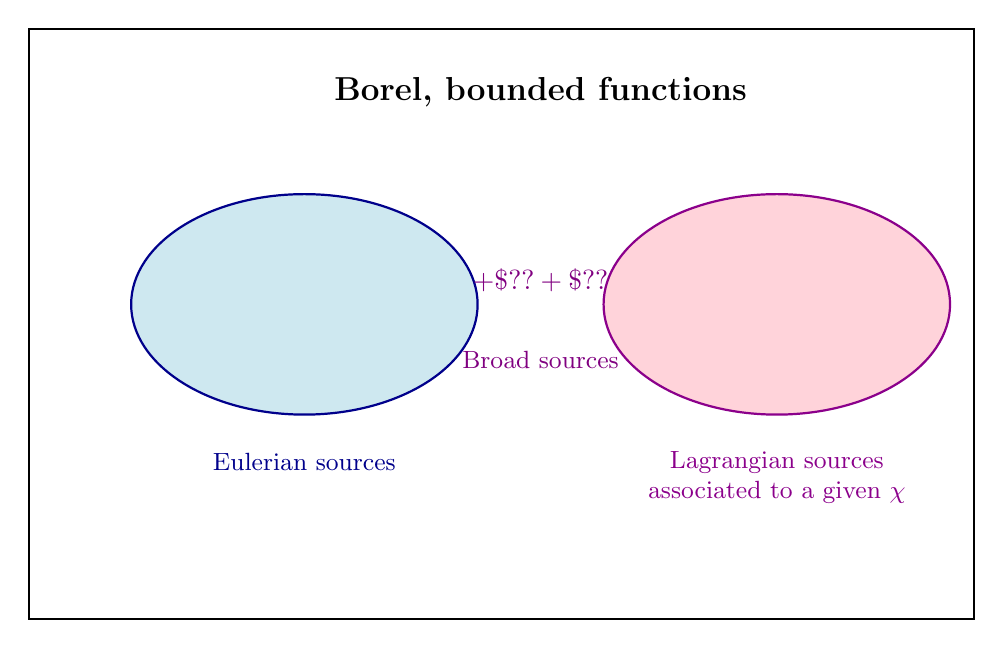
\begin{tikzpicture}[scale=1]

    % Frame
    \draw[thick] (-1,-0.5) rectangle (11,7);

    % Title
    \node[anchor=north, font=\large\bfseries] at (5.5,6.5) {Borel, bounded functions};

    % Left ellipse (Eulerian sources)
    \filldraw[darkblue, thick, fill=lightblue, fill opacity=0.6] 
        (2.5,3.5) ellipse (2.2cm and 1.4cm);

    % Right ellipse (Lagrangian sources)
    \filldraw[darkmagenta, thick, fill=lightpink, fill opacity=0.6] 
        (8.5,3.5) ellipse (2.2cm and 1.4cm);

    % Intersection notation
    \node[purple] at (5.5,3.8) {$+\$ ?? +\$ ??$};
    \node[purple, font=\small] at (5.5,2.8) {Broad sources};

    % Left label
    \node[darkblue, font=\small] at (2.5,1.5) {Eulerian sources};

    % Right label
    \node[darkmagenta, font=\small, align=center] at (8.5,1.3) {Lagrangian sources\\associated to a given $\chi$};

\end{tikzpicture}

\end{document}